%%%%%%%%%%%%%%%%%%%%%%%%%%%%%%%%%%%%%
% This file is the "main" or root file for the book. It describes what packages
% and content should be included in what order.

\documentclass[pagesize=auto,bibliography=totocnumbered]{scrbook}

\usepackage{comment}
\usepackage{etoolbox}
\usepackage{fancyvrb}
\usepackage{graphicx}
\usepackage{hyperref}
\usepackage[round]{natbib}
\usepackage{xspace}
\usepackage{xcolor}

% This is for multilingual work. Would be nice to support Chinese and Thai.
% \usepackage[T2A]{fontenc}
\usepackage[utf8]{inputenc}
% \usepackage[greek,russian,english]{babel}

\usepackage[T1]{fontenc}
\usepackage[english]{babel}

% This file is for commands / macros / functions.

% That at least was the original intention. As you can see from the comments, some of the commands
% that work for TeX and pdf output are innefective when applied to HTML and eBooks!

% These are useful because HTML output corrupts the result of the \latex command.
\newcommand{\latex}{LaTeX\xspace}
\newcommand{\tex}{TeX\xspace}

% Makes extra space in HTML but not in PDF output.
\def\htbr{\ifdefined\HCode{\HCode{<br/><br/>}}\fi}

\newcommand\nextpage[1][]{
\ifdefined\HCode {
  \HCode{<mbp:pagebreak />}}
\else
  \newpage
\fi
}

% Makes small typewriter text, comparable to other font sizes.
\def\smalltt#1{\texttt{\small #1}}

% Makes small verbatim inline typewriter text, comparable to other font sizes.
% Use as \sverb|My verbatim text|
\def\sverb{\Verb[fontsize=\small]}

% Makes small URL text, comparable to other font sizes.
\def\surl#1{{\small{\url{#1}}}}


% This line stops the insertion of extra blank pages between chapters.
\ifdefined\HCode{\KOMAoptions{twoside=false}} \fi

\begin{document}

% Title and author are written down in the cover_page.tex file, and author
% appears also as an argument to the ebook-convert command in the build.sh file.
%% This is a cover page.

\thispagestyle{empty}

\vspace{3cm}
  \begin{center}
	\bfseries \Huge \latex to eBook 2021 \par   % Your own title would go here.
        ~\\
	\bfseries \LARGE The Book About Itself \\   % Include a subtitle or just delete.
        ~\\
        \bfseries \Large Dominic Widdows \par   % The author's name goes here.

        \vspace{3cm}
    
      	{\centering 
\includegraphics[width=0.8\linewidth]{images/cover.png}}
    \end{center}
    
\par

\newpage


\tableofcontents

\nextpage
% %% Introduction / first chapter.

\chapter{Introduction to \latex and eBooks}

Considering writing a book? Good for you! Publishing a book is easier and cheaper today 
than it ever has been. 

If you know what you want to write about, the next step (and sometimes the 
hardest step) is getting started. The most important part is the material itself: 
you can write paragraphs in any number of text and document editors, 
and figure out how to format the material as a book later. But sooner or later, 
the question arises of how to turn the material into a book format. That could mean a paper book, 
which requires physical resources for printing and distributing. Or it could mean
an eBook, to be read on an eReader such as an Amazon Kindle or Kobo
Clara, or using an app on a phone, tablet, or laptop.

So how do you turn your document into an eBook? This is a very short book demonstrating one 
way to do this, and if you're reading this on an eReader, that shows
that it already worked at least once --- for this book.

To start with, I chose to use the \latex typesetting system. 
The original \tex was created by the famous computer scientist Donald Knuth \citep{knuth1984texbook},
and added to by Leslie Lamport to make \latex \citep{lamport1985latex}.
\latex is used throughout scientific fields to write papers and books. There are many
reasons for preferring \latex to one of the more `point, click, and type' text editors:
it handles figures, tables, chapters, sections, headings, cross-references, 
bibliographic references, mathematical equations, and many more things that can be 
notoriously irritating and time consuming to get right. And it's possible to use different typesetting
programs and commands to create all sorts of output from \latex input, including eBooks.

If \tex and \latex are entirely unfamiliar to you, even this automation and flexibility 
may not make it the best choice for you to write a book, because there is quite a technical 
learning-curve for \latex. It's not just writing text, it's writing commands telling the
typesetting program how to `compile' the output document --- in many ways, \latex
feels much more like programming than writing a Google or Microsoft Word document. But if
\latex is something you've already used to write a dissertation or paper, you're 
probably well aware of its benefits (and its hassles). 

In summary, if you've used \latex to write papers, now you want to write an eBook,
and you need to figure out how to do this, then this little book and
the open source template that it comes from might be ideal.
There are other ways to make eBooks, and other ways to use
\latex to make eBooks --- this book isn't comprehensive, but it might just
enable you to make an eBook end-to-end quickly, cheaply, and easily.

%%%
\section{How to Use this Book}

This is a book about itself --- it's about how it was written using
the templates and tools described in 
the next few chapters. These are the main ways you can use this material:

\begin{itemize}
    \item You can read it. It shouldn't take long, it outlines the process
    used to make this eBook end to end, and then you can decide if this is something you want to try.
    \item You can use it as an instruction manual, learning and following some of the procedures step-by-step to make your own book.
    \item You can use it as a template. All of the source files used to make this book
    are freely available in GitHub at {\small \url{https://github.com/dwiddows/ebookbook}} and Overleaf.
    The source files are laid out in a way that should make it easy to clone the project and adapt it for your own book.
\end{itemize}

It follows that you could recreate this eBook for yourself, following just the process
described in the book: which is basically to clone the GitHub project as a template, build
the project, send the output HTML document through an ePub converter, and send this to
your eReader device.

So why would anyone buy a book if it's free? Because
anyone who reads the steps above and with enough familiarity to think
``git clone \ldots check dependencies \ldots  build.sh \ldots 
check dependencies again \ldots build.sh \ldots  \ldots yeah, alright'' will expect it to take
more than a few minutes, hopefully less than an hour, and price their own time realistically.
If you want to read this book for free on your eReader,
compiling from source is the way to go about it. Or if you want to just click `buy' now and send the author most of the
\$2.99 price tag, please go ahead, and thank you!

Either way, if you're not put off by \latex and \smalltt{git}
commands, keep reading. I hope the book is useful to you, and wish you 
all the best of luck and persistence writing your book!
 
% % The end to end process: second chapter.

\chapter{End to End: From Source to eReader}

We'll start with the end-to-end process for making a book you can read
on your eReader device. Once you can do this, change the title,
add or remove chapters, and see the changes you've made reflected on your 
eReader, that will hopefully be the best encouragement to take the
parts that are most useful and get started with your own book.
The basic outline of the process is shown in Figure \ref{fig:pipeline}.
The rest of this chapter walks through the steps in more detail.

\begin{figure}
\begin{center}
  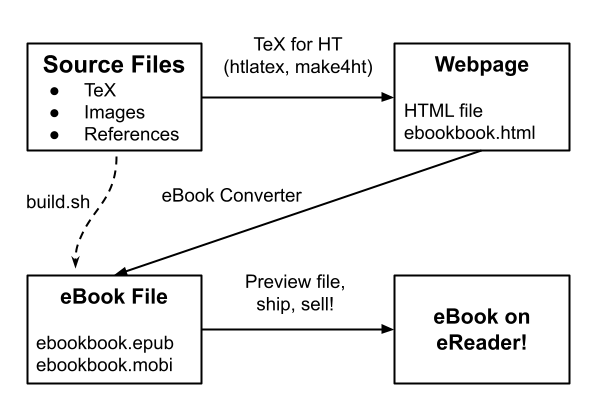
\includegraphics[width=\linewidth]{images/process.png}
 \vspace{0.2cm}
\caption{Steps in the pipeline for shipping this eBook}
\end{center}
\label{fig:pipeline}
\vspace{0.4cm}
\end{figure}

%%
\section{Install Dependencies}

Typically when you want to use a new piece of software, it has
dependencies --- other libraries and packages it needs for some of its
functionality. For end-user applications, these are usually bundled
together so that everything works `out of the box'. For programming
tools, there's normally some system to check which dependencies you
already have, and to install only the new ones that you need. How this
works depends partly on what platform you're using. Here we'll just list
the dependencies you'll need to find and install.

These include:

\begin{itemize}
\item A \latex system, including a program called \smalltt{make4ht} or the older \smalltt{htlatex}.
  This is crucial for making HTML output, as described in Section
  \ref{sec:html2epub}.
\item Some eBook converter software. The one recommended below is
  \smalltt{ebook-convert}, from Calibre (see
  {\small \url{https://manual.calibre-eBook.com/ebook-convert.html}}, or just
  search the web).
\item Some eReader or previewer software, such as a Kindle device or
  app, or another eBook app such as Calibre (see above). You'll want
  this for seeing how your book looks `for real' (though of course,
  not all eBook apps look exactly alike, and users have different settings).
\item (Recommended) A shell program that runs bash scripts so that you
  can run the \smalltt{build.sh} command. If you don't already have a
  terminal where you can run bash or a close equivalent, it's probably
  worth installing and using, and if that instruction sounds
  difficult, the rest of the process may be hard.
\end{itemize}

Every modern operating system --- basically Windows, Linux, MacOS, and
similar variants --- has a variety of package installation tools.
Some of the dependencies above can be done at the command-line, sometimes it's
easier to download and install something directly from a provider's
website.

The best place to keep links to such dependencies and recommended options is the 
github project wiki at {\small \url{https://github.com/dwiddows/ebookbook/wiki}}.

%%
\section{Access and Build the \latex Source}

Next, you'll want to get a copy of the source code for this
book. (\latex sources count as
`code' for these purposes. It gives instructions to machines, it's easy to make mistakes
that show up as error messages, and it's reviewed and stored in source
control --- so it's like code in these practical senses.)

If you already have \smalltt{git} installed, this will be something
like running \smalltt{git clone
  https://github.com/dwiddows/ebookbook.git} at a command prompt, or
downloading the code using some visual client software. 

List the contents of this directory and check that you can see the
files \smalltt{ebookbook.tex} and \smalltt{build.sh}. The first of these
is the main \tex document that lays out how to combine the other files
into an eBook.  The second is a build script --- on platforms with
bash or a compatible shell installed, you should be able to run just
\smalltt{./build.sh} and get most of the book built using one
command. Or at least, to begin with, you should get error messages
telling you if anything is missing and needs to be installed. If you're not
running a compatible shell, the \smalltt{build.sh} file at least lists
the commands you'll need to run some other way.

So the next step is to run \smalltt{./build.sh} and ideally it should
typeset a copy of this book. If the \smalltt{ebook-convert} command is
available it should even make the eBook files described in the next
section.

If this doesn't work, you may need to find and install some
\smalltt{pdflatex} and most importantly \smalltt{make4ht} or
\smalltt{htlatex} programs that work on your machine. (See the
Dependencies section above.)

So long as you can run ``\sverb|make4ht ebookbook|'' and create a file \sverb|ebookbook.html|,
you can go on to the next step.

%%
\section{From HTML to ePub ... or Mobi}
\label{sec:html2epub}

The most important output from the previous step is a file called
\smalltt{ebookbook.html}.  This is formatted for display as a webpage
in a browser. This is different from the more common use of \tex to
make documents such as academic papers, which are nowadays normally
created as PDF files. An HTML file is a collection of content (for
example, words and images to display), and typesetting suggestions
(for example, make this text a heading, and make this image 40\% of
the screen width). By contrast, a PDF file has
precise instructions about how big to make each character and which
page to put it on. So it makes sense that HTML is more like an eBook:
instead of saying what text will appear on which page, it gives
directives about what text should be bigger and smaller, and this
combines with the user's device settings to decide which page it
should appear on.

So the \smalltt{ebookbook.html} file (rather than the corresponding
PDF file or any other page-layout format) will be used to
create your eBook format. 

You can turn your HTML file from a webpage into an eBook by installing
and using a converter such as Calibre \smalltt{ebook-convert} or
Amazon's {\em Kindle Previewer} tool.
Like saving an image as a
\smalltt{.jpg}, \smalltt{.gif} or \smalltt{.png}, you'll need to select a
format to convert to. Options include:

\begin{itemize}
  \item \smalltt{.epub} is a cross-platform format that it supposed to
    be used for any electronic book.
  \item \smalltt{.mobi} is an old Amazon Kindle format --- and it
    happens to be the one you can use for e-mailing files to your Kindle.
\end{itemize}

The \smalltt{build.sh} script that comes with this book uses
\smalltt{ebook-convert} and creates both \smalltt{.epub} and
\smalltt{.mobi} files as output. This also takes command-line
arguments so that you can specify metadata like the author name
and cover image:

{\flushleft \quad \smalltt{ebook-convert ebookbook.html ebookbook.epub --cover images/cover.jpg --authors "YOUR NAME" --language English}}

%%
\section{Previewing Your Book on an eReader}

Hopefully by now you have an eBook. Or at least, a file called something like
\smalltt{ebookbook.epub}. So how do you {\em read} your book?

For this you'll need an eReader --- perhaps an app on your computer or phone,
or an eReader device such as a Kindle.

Assuming that most of your writing will be on a computer, that's
probably the first place you'll want to see your work. For example, I
usually open the Calibre app and load the \sverb|.epub| file, or do both at
once with the command \smalltt{calibre ebookbook.epub}. Once the book is imported and loaded, this gives 
the result shown in Figure \ref{fig:calibre_screenshot}.

\begin{figure}
  \begin{center}
    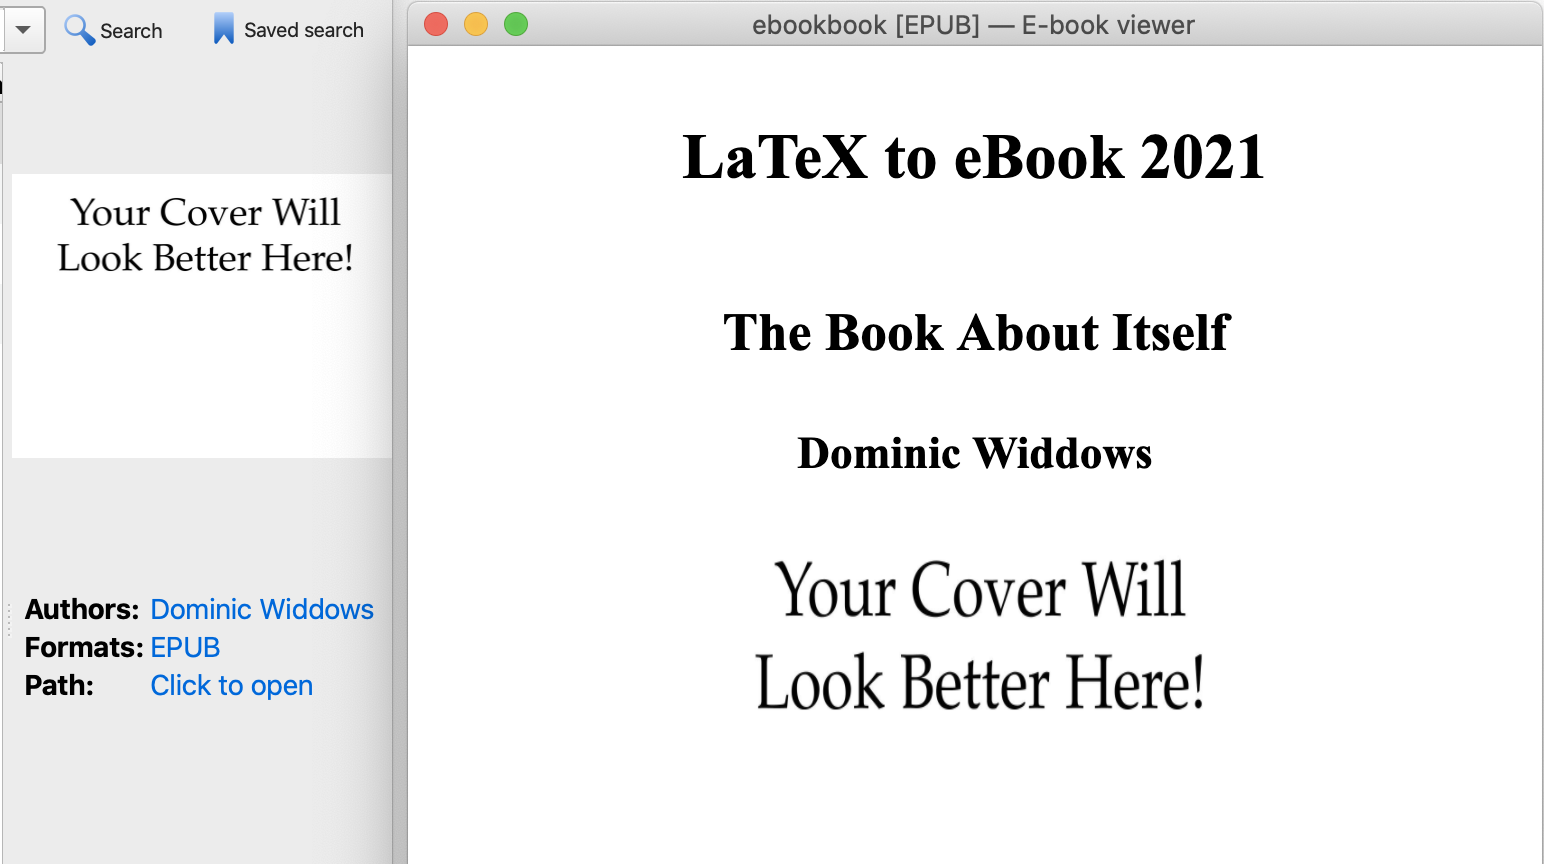
\includegraphics[width=\linewidth]{images/calibre_screenshot.png}
    \htbr
    \caption{Thumbnail image and cover page in Calibre}
\label{fig:calibre_screenshot}
\end{center}
\end{figure}

To view on an eReader device or phone, you often have to send it to
the device or load it on in some way --- again, there are a range of
methods. For Amazon Kindles, you need to find / set up an email address for the
device itself, and send the book to that email address. As an extra
complexity, this method only works using the older \smalltt{.mobi}
files.  Also Kindle preloads like this do not (at the moment)
display the cover page of the book in your library or menu page,
because Amazon retrieves this information for {\em published} books
from elsewhere. So the preview in the library view is somewhat
disappointing, but it works (Figure \ref{fig:kindle_screenshot}).

Another way is to sign up for a publishing account and start to submit your book for
publication. On the Kindle publishing site, for example, this process includes opportunities
to preview your book as it would appear on a phone and a Kindle device, before you set up
pricing options and get closer to hitting `publish'. For this book at least, these online previewers
gave a more accurate rendering of how the book will look to readers than emailing a \smalltt{.mobi} file to my
Kindle device.

One way or another, try to make sure you can make an eBook file and view it somewhere.

\begin{figure}
  \begin{center}
  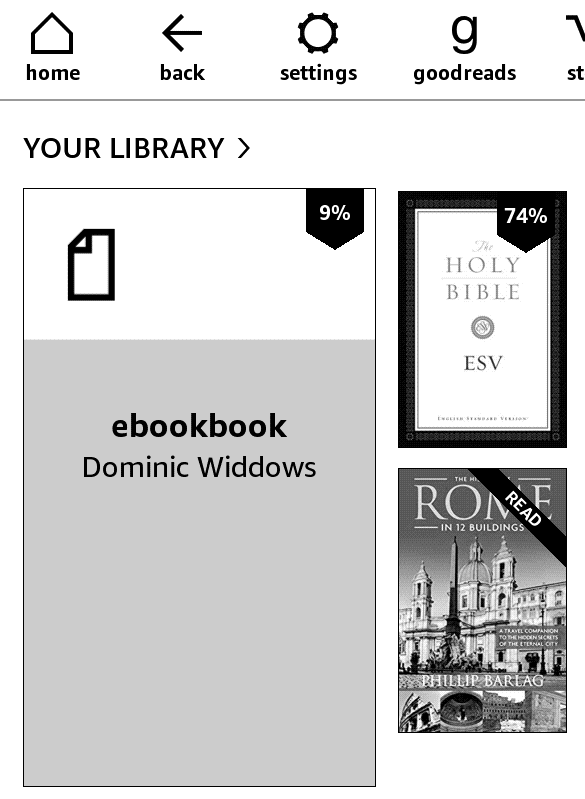
\includegraphics[width=0.6\linewidth]{images/kindle_screenshot.png}
  \htbr
  \caption{Book thumbnail image loaded onto a Kindle}
  \label{fig:kindle_screenshot}
 \end{center}
\end{figure}

%%
\section{Make it Your Own!}

Hopefully by now you're at the point where there is an eBook file that you can easily read on some eReader device or app. 

The next thing you should do is change something. Change the title in the \smalltt{cover\_page.tex} file from `\latex to eBook 2021'
to whatever title you want. Rerun the steps above and hopefully you'll see exactly what you intended: a copy of the eBook, but with
your title instead.

At this point you're off to the races. That doesn't mean that it's all plain sailing from here: there will likely be glitches and hurdles along the way.
But the main thing is that you have a template, examples of several \latex constructs that work with eBooks, and you're able to start turning this
into your own book. You may want to save your work separately at this point, call the project something else, and if you use source control,
start checking in your work in some way that makes it clear that it's a new project, rather than a work-in-progress on the old project that's intended to be
merged back in at some point.

Experiment with removing directives to \sverb|\input| different chapters, and watch the book get shorter. Try changing image files to some other graphic
and make sure they change appropriately. And try editing the AUTHOR in the \smalltt{build.sh} file and make sure the right name shows up when the book is viewed in an eReader.

If this works, you can be pretty confident that your book is on the right track. You'll be able to organize the content into \tex files, image files, etc., and create an eBook!


%%%
\section{Publication}

Nearly all of this book is about how to create and preview eBook files, and this is like a software development process
--- you should be able to run the pipeline over and over again and keep testing that the change you made had the desired effect.

Publishing and marketing your book is a different process: you'll be using an online browser app, signing up for accounts, uploading files, filling in forms,
you'll eventually click "submit", and hopefully see your book available for download / purchase after a short while (in the case of this book, a few hours).
Look for opportunities to preview your book as part of the submission process.

This process with Amazon Kindle has was straightforward enough form-filling. You can upload your own cover image, or use the online tools
to create one. Submission for publication brings up questions like pricing and (related) copyright agreements. To claim a 70\% royalty for original work,
rather than a 35\% royalty, Amazon says you have to price your book between \$2.99 and \$9.99. Hence the \$2.99 price tag for this book.

It takes at least a few hours before your book is live and available --- and it may take longer to start appearing in search results.

Note that you can upload new versions of your book any time. Updates (at least minor ones) get automatically processed and released
in just the same way as the initial submission. With this book, for example, I submitted two revisions within a few hours, because of
course once I was viewing the book `for real' on my phone, there were a couple of typos and small mistakes I wanted to fix.
So in the case of this book, I published it and updated the live version a few times before even telling people it was available.

If you found this book in the Kindle store and can read this as a result, it worked. And if I could do this, you can too!






% %%
\chapter{Typesetting Topics}
\label{chapter:typesetting}

This chapter will go through some of the \tex features you'll probably want to use at some point.
So far, {\em most} of the things I usually do with \tex can be made to work for eBook outputs,
but there are lots of commands and options that don't work and you need to know which
variants to use.

%%
\section{References and Citations}

One of the easy things that `just works' most of the time in \latex is references. For example,
the \tex source for this chapter starts with:

\begin{Verbatim}[fontsize=\small]
\chapter{Typesetting Topics}
\label{chapter:typesetting}
\end{Verbatim}

Then if I want to refer to the chapter, I write \sverb|Chapter \ref{chapter:typesetting}| which
gets rendered as `Chapter \ref{chapter:typesetting}'. Adding \smalltt{label} commands for tables and figures
works in the same way.

This isn't rocket science, but if you've ever tried
renumbering by-hand, you know how valuable this is! Similarly, bibliographic references such as
\sverb|\cite{knuth1984texbook}| work correctly, giving a citation looking like \cite{knuth1984texbook}.
So far \textsc{BibTeX} has worked fine for this book.

%%
\section{Graphics}

Nearly all eBooks have graphics in them somewhere, even if just for a cover page. 
The \smalltt{graphicx} package works well for this.
For example, the cover image for the title page of this book is included using the command:

\begin{Verbatim}[fontsize=\small]

\includegraphics[width=0.8\linewidth]{images/cover.png}
\end{Verbatim}

Typically for webpages and eBooks, the size of images is expected to vary with the page size and settings,
so using a context-sensitive width like a proportion of the linewidth is more appropriate than a fixed-width
declaration like `10cm'. Many eReaders enable users to click on images to see them in more detail, which helps.

One frequent problem is that HTML typesetting using \smalltt{make4ht} or a similar process doesn't always preserve the
aspect ratio of your images. For example, the same setting may be used for width and height, making all images square.
The problem is solved by adding a bounding box file using the \smalltt{extractbb} command, which is typically included
with \tex distributions. For this book, this step is included in the project's \smalltt{build.sh} script, at least for \smalltt{.jpg} and
\smalltt{.png} files, and it can easily be extended to more filetypes. Or you can run \smalltt{extractbb -x} on these files
yourself.

Images are often put in the \latex \smalltt{figure} environment, which can include captions and a label for references.
For example, the map in Figure \ref{fig:sea_map} is created using the commands:

\begin{Verbatim}[fontsize=\footnotesize]
\begin{figure}
\begin{center}
  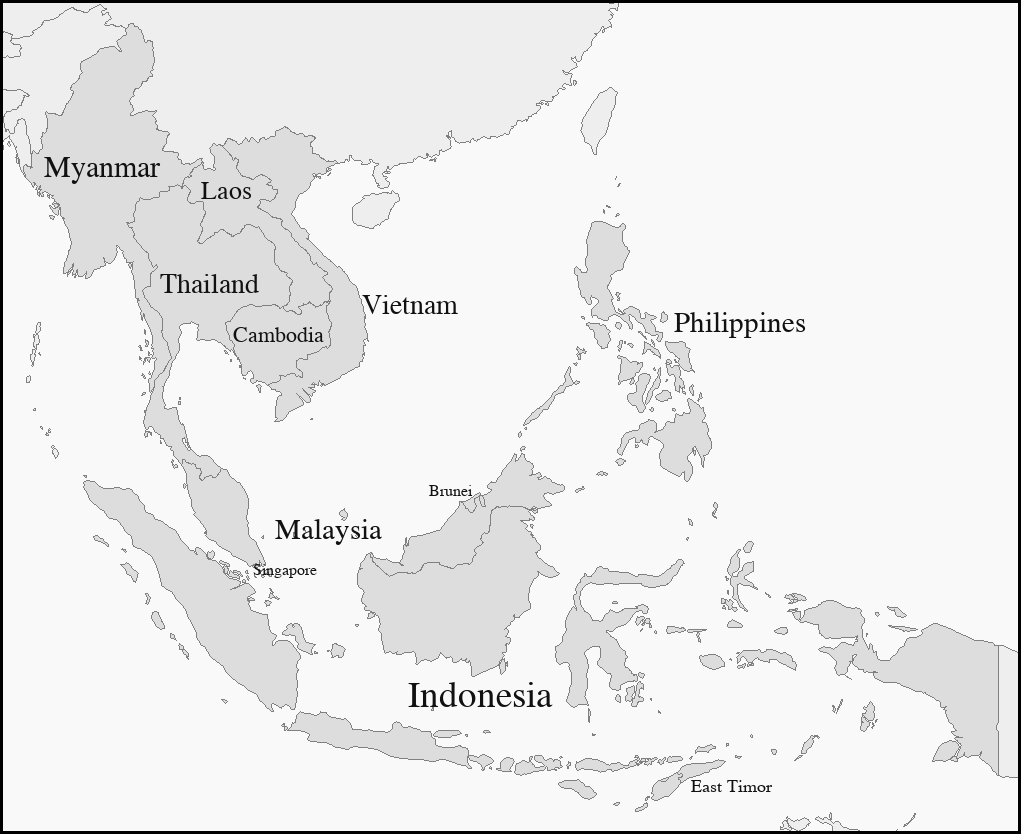
\includegraphics[width=\linewidth]{images/sea_countries.png}
  \htbr
  \caption{Map of countries in Southeast Asia}
  \label{fig:sea_map}
\end{center}
\end{figure}
\end{Verbatim}
  
\begin{figure}
\begin{center}
  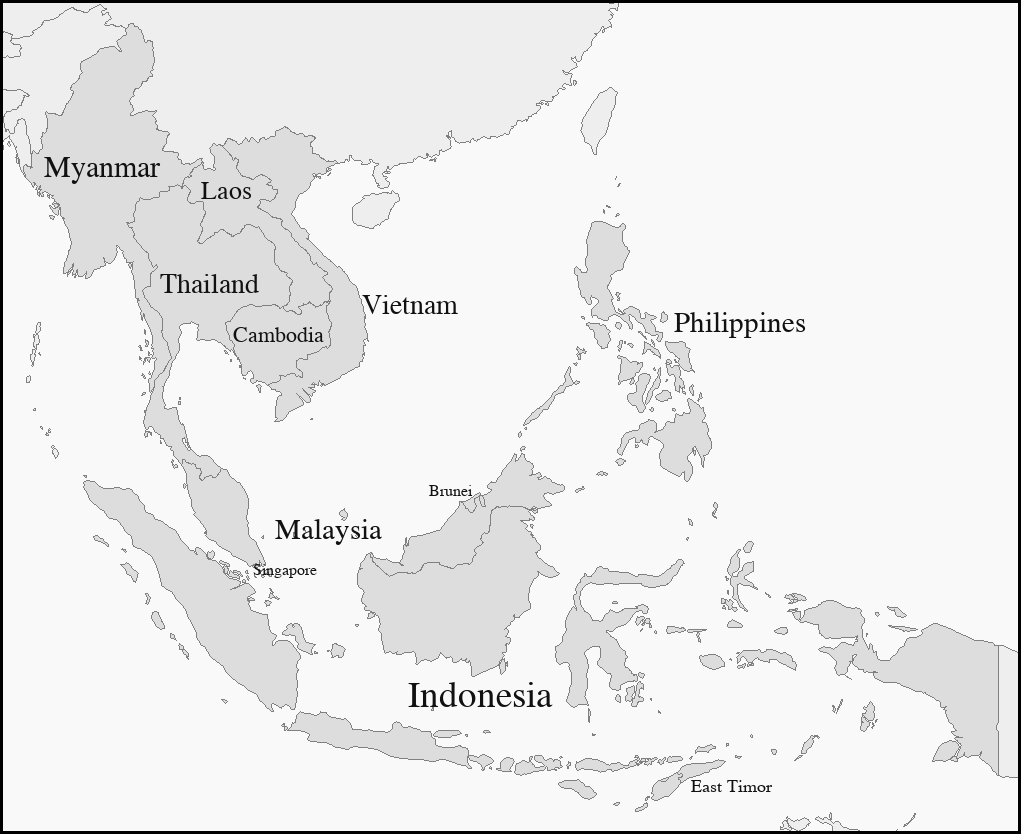
\includegraphics[width=\linewidth]{images/sea_countries.png}
  \htbr
  \caption{Map of countries in Southeast Asia}
  \label{fig:sea_map}
\end{center}
\end{figure}

Note the \sverb|\htbr| command, which is defined in the macros as
\sverb|\ifdefined\HCode{\HCode{<br/><br/>}}\fi}|.
This is an extra \tex command for hypertext: it forces
some vertical space to be included between the image and the caption, because the usual \tex command
\sverb|vspace| seems to have no effect on the HTML (and hence ePub) output here.

From here, the figure can be referenced using the command 
\sverb|\ref{fig:sea_map}|. (Made using \surl{https://github.com/dwiddows/pilmaps},
a free mapping tool in python that supports low-level, hands-on rendering control --- feel free to try it out.) 
So far I haven't found an effective way of controlling the placement of figures --- for example, directives
like \sverb|\begin[ht]{figure}| don't affect the HTML or the ePub output, and I haven't got
wraparound text to work.

 %%
\section{Tables}

Basic tables typeset just fine in \smalltt{.epub} format. They don't format properly in the Kindle preview of \smalltt{.mobi} files
sent via email, but look better in the Kindle \smalltt{.epub} preview.

For example, the following \latex gives the output in Table \ref{tab:artist_works}.

\begin{Verbatim}[fontsize=\footnotesize]
\begin{table}
  \centering
  \begin{tabular}{|c|l|}
    \hline
    \textbf{Artist} & \textbf{Great Works} \\
    \hline
    Leonardo da Vinci & The Mona Lisa \\
    Charlie Watts & Satisfaction \\
    \hline
  \end{tabular}
  \caption{Inspiring works}
  \label{tab:artist_works}
\end{table}
\end{Verbatim}

\begin{table}
 \centering
  \begin{tabular}{|c|l|}
    \hline
    \textbf{Artist} & \textbf{Great Works} \\
    \hline
    Leonardo da Vinci & The Mona Lisa \\
    Charlie Watts & Satisfaction \\
    \hline
  \end{tabular}
  \caption{Inspiring works}
  \label{tab:artist_works}
\end{table}

With standard \latex it is easy to make tables that are too big for pages or that typeset poorly for other of reasons.
I expect this can be even more of a problem with small-screen eBooks, so you'll want to design any tables accordingly
and check output carefully.

%%
\section{Equations}

One of the benefits of \latex is that it's easy to typeset mathematical notation like formulae and equations. So far these look to work well in HTML and eBook formats.

For example, here is the \tex and its rendering for Euler's formula:

\begin{Verbatim}[fontsize=\scriptsize]
\[ e^{ix} = \cos x + i \sin x \]
\end{Verbatim}
\[ e^{i\pi} = -1 \]

And here is the corresponding \tex and output for a Fourier series:

\begin{Verbatim}[fontsize=\scriptsize]
\[ f(x) = \sum_{k=0}^{\infty} [  a_k \sin(kx) + b_k \cos(kx) ] \]
\end{Verbatim}
\[ f(x) = \sum_{k=0}^{\infty} [  a_k \sin(kx) + b_k \cos(kx) ] \]

Array environments for typesetting rows and columns in equations also work, for example:

\[
u = \left( \begin{array}{c} 1 \\ 0 \\ -2 \end{array} \right) \qquad
v = \left( \begin{array}{c} 2 \\ -1 \\ 3 \end{array} \right) \qquad
u^T v = 2 + 0 - 6 = -4 \qquad
u v^T = \left( \begin{array}{ccc} 2 & -1 & 3 \\ 0 & 0 & 0 \\ -4 & 2 & -6 \end{array} \right)
\]

This set of equations may become typeset in a smaller font than those above, to fit them
horizontally on a small screen. If these start to get too small, consider breaking lines up
when typesetting mathematics for eBooks.

%%
\section{Different Languages}

It's possible (and sometimes easy) to typeset documents using languages other than English
and character sets other than the Latin alphabet.

For example, this is in Russian:
\selectlanguage{russian}
Это на русском.

\selectlanguage{english}
This is in Greek:

\selectlanguage{greek}
Αυτό είναι στα ελληνικά.

\selectlanguage{english}
These examples are made using the \sverb|babel| package, and by setting
encoding instructions in the initial document setup (see the \sverb|lib/packages.tex| file),
and then in the \latex source writing something like:

\begin{Verbatim}[fontsize=\footnotesize]
This is in Greek:
\selectlanguage{greek}
( add your text here )

\selectlanguage{english}
This is back in English.
\end{Verbatim}

I have not got Chinese or Thai working properly yet. There is an example file in \sverb|tests/languages.tex|
showing this.

%%
\section{Contents and Index}

The table of contents should get typeset automatically if you use this template.

The story of how traditional indexes and concordances influenced the design of the inverted
indexes used by search engines is fascinating \citep[Ch 1]{witten1999gigabytes}.
For electronic books, this process is quite complete: the index is created automatically,
and accessed via the search interface, not by the user scrolling through topics in alphabetical order.
Therefore I'm not including an explicit index section.

If you want to make a paper
version of your book as well as an eBook, you may want to make an alphabetical index.
In this case, it may be worth trying a
more sophisticated template such as the one that comes with Clemens
Lode's book on using \latex for books and eBooks \citep{lode2019better}.
This includes conditional compilation so that different commands and even sections are used
for the PDF version that leads to a paper book and the HTML version that leads to an eBook.

%%
\section{Difficulties}

Several things have proved tricky and may just not work with typesetting to HTML.

Exact placement is sometimes impossible. Figures, tables, and captions may appear
in various places, and often don't obey \tex typesetting directives. For example,
putting an \sverb|fbox| (framebox) around a figure makes it float to the left, irrespective of
centering commands. Captions may easily fall across
a page boundary, so one tip is to keep captions small (one line), just enough for the reader
of the main text to see that they are looking at the right table or image.

Controlling font size in different environments has been hard, particularly with typewriter fonts
used for verbatim text such as rendering \latex commands that you don't want to be interpreted as
\latex commands. In retrospect, trying to write an eBook about \latex itself was perhaps not the
most sensible decision! But this has been fixed using the right combination of commands from the
\sverb|fancyvrb| package, included here as macros like \sverb|\sverb| for `small verbatim' and
\sverb|\surl| for `small URL'.

Some of these things lead to useful design considerations.
Remember that we're designing for a small screen, whose font size and spacing is up to the user. 
Don't struggle to make a particular page look perfect on your device
only to see later that for someone with a larger font setting, this content is broken across
several pages. Try to make your book design clear, legible,
and somewhat flexible, and a huge variety of readers will be able to enjoy it!


% %%%
\chapter{Maintenance and Troubleshooting}

We're nearly done with this short template book --- at least with the first version.
But as with most topics to do with software and electronic information, things will keep changing.
Bugs will hopefully get fixed, new bugs will arise, different devices will support different formats,
standards may change --- for example, it may become
possible to load \smalltt{.epub} files directly onto an Amazon Kindle, rather than having to use the
\smalltt{.mobi} format solely for this purpose. This last chapter will include a few suggestions on how
to ask questions and report changes.

%%
\section{Report Bugs on Github}

The open source github repository for this project is {\small \url{https://github.com/dwiddows/ebookbook/}}.
If something recommended in this book doesn't work for you, and if you have to change or add extra
commands to make it work, please report this as an issue there. The github project wiki can be used for
keeping instructions up-to-date and adding links to more resources. This is likely to be much more effective
the reporting problems on sites where the book is sold.
If you want to review the book itself, post a review. But if you want to report a problem and get
help, please use the project github site.

When there are major developments or enough new things to include, I will add these to future
editions of this book (if there are any!). But by design, books are meant to be relatively stable, whereas
project websites and wikis are designed to have immediate updates. If a new `edition' comes out too often,
we can lose track of what to refer to.

So tl;dr: please leave actual reviews on marketplace sites, but report bugs on github. Not just because
I want to avoid a bunch of frustrated bug reports as book reviews, but also because if
bugs are reported on the github project, they're more likely to be addressed and fixed!

%%
\section{That's All For Now}

This was always intended to be a short book, just enough to provide a working template, to demonstrate
a few typesetting features, and to make the book whose end you're just reaching.

I hope it's given you some confidence to get started, and in particular, I hope the structure works for you.
Clone the project, install a few dependencies, try it out, and ideally within a short time you won't be thinking
much about this book --- it will already be becoming {\em your} book.

Good luck and enjoy your writing!

\begin{flushright}
  {\em Dominic Widdows \\ September 2021}
\end{flushright}






\nextpage

% After the \backmatter command, sections will not be numbered.
\backmatter

%%
\chapter{About the Author}

Dominic Widdows is a mathematician, computational linguist, and software engineer.
He has worked on differential geometry and Oxford, natural language processing at Stanford,
and many projects at MAYA Design, Google, Microsoft, Grab, and LivePerson, where he works
particularly on conversational AI and internationalization.

As an author, his work includes the book \href{https://www.amazon.com/-/dp/B00J4FZOOY/}{Geometry and Meaning},
and over 50 scientific papers, in areas including pure mathematics,
computer science, language processing, bioinformatics, information extraction, logistics, and quantum computing.
As a developer, his open source contributions include work on the
\href{https://github.com/sky-map-team/stardroid}{SkyMap Planetarium App},
the \href{https://github.com/semanticvectors}{SemanticVectors} project, and
\href{https://github.com/dwiddows/pilmaps}{PILMaps} for drawing maps.

Enthusiasm for scientific publishing and open source development combined to make this book. 






\bibliographystyle{apalike}
\bibliography{bibliography.bib}

\end{document}
